\section{Mizar}

\begin{minipage}{0.5\textwidth}
\textbf{Name}: Mizar\\
\textbf{Function}: The Antagonist, the Evil Stepmother

\subsection{Internal World}

\textbf{Age \& Gender}: about 200, female \\
\textbf{Values \& Virtues}: Vengeance \\
\textbf{Personality}: Manipulator, heartless, egocentric, vindictive \\
\textbf{Interests}: Magic, king of Ingary \\
\textbf{Ethnic Group}: Arabic djinn

\subsection{External World}
\textbf{Environment}: Castle of Dynamia, Kazan island \\
\textbf{Education}: High-educated, magic \\
\textbf{Social \& Cultural Background}: Each people in Strangia respects her because they fear her power. Nobody knows the real reasons why the war is going on. Nobody knows the real story of Mizar \\
\textbf{Look \& Feel}: She is about 200 years old but she looks like a 30-35 years old woman. She has pointy ears  \\
\textbf{Job \& Experience}: Court magician, Queen regent \\

\end{minipage}%
%
\hfill\begin{minipage}{0.4\textwidth}
  \begin{figure}[H]
  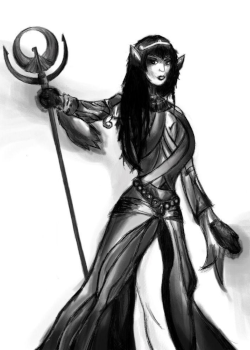
\includegraphics{Images/Characters/mizar_portrait}
  \caption{Sketch of Mizar made by Elena Coperchini}
\end{figure}
\end{minipage}

\subsection{Relationships}
\begin{itemize}
\item \textbf{Sophie}: She didn’t know Sophie until she tries to defeat her. Since then, Mizar hates her.
\item \textbf{Howl}: She knows him just by reputation but she has never met him until he tries to defeat her. Since then, Mizar hates him. She fears him a bit because rumors say that he is a powerful wizard.
\item \textbf{Calcifer}: She hates him because he is a friend of Sophie and Howl.
\item \textbf{Justin}: He is her stepson. She gets him arrested only because he is a bare  inconvenient with her plans. 
\item \textbf{Suliman}: Mizar has only heard about her, but she still hates her because she is the new court magician of Ingary.
\item \textbf{Belzel}: They don't know each other.
\end{itemize}

\begin{figure}[H]
  \centering
  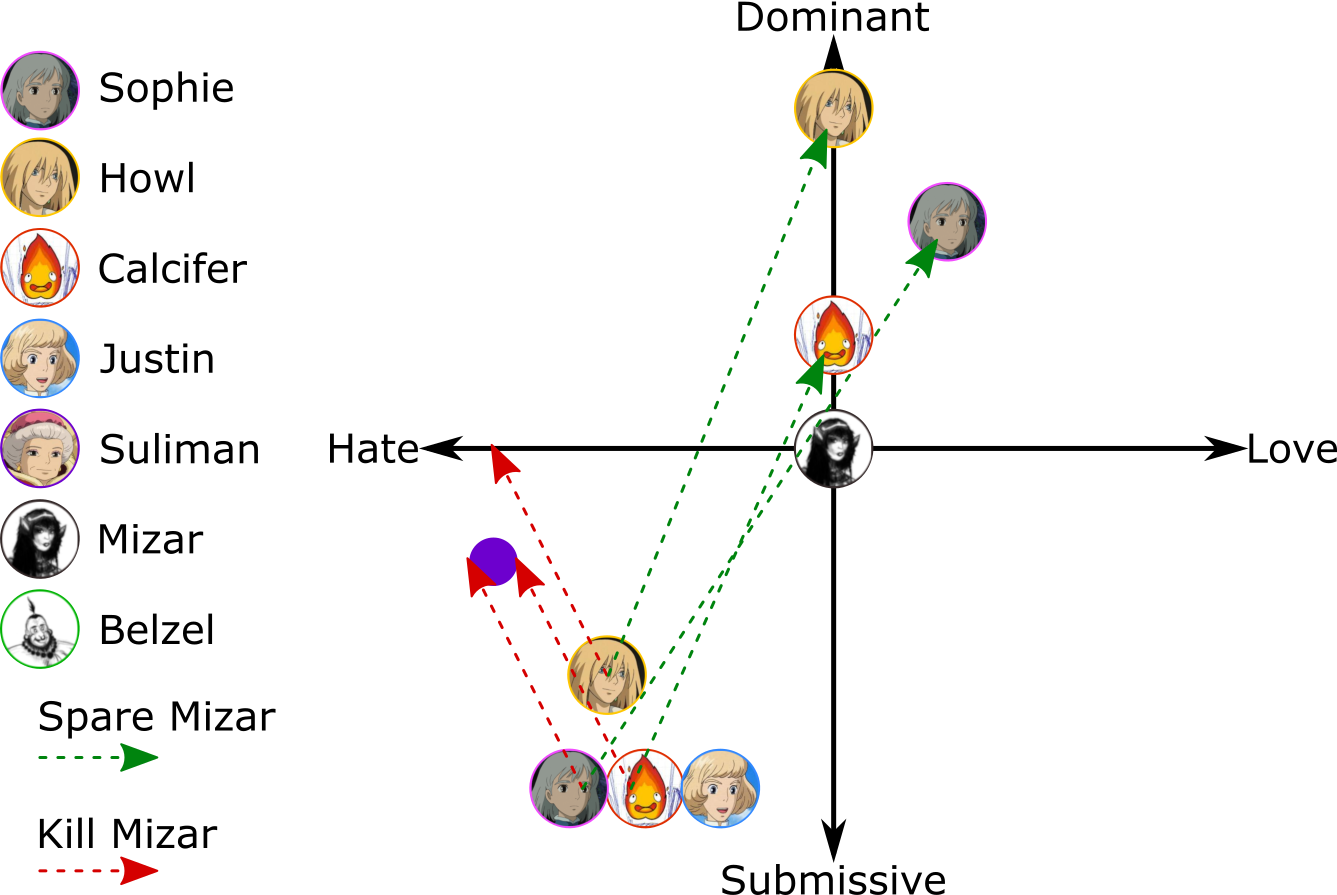
\includegraphics[width=14cm]{Images/Diagrams/Circumplexes/mizarCircumplex}
  \caption{Circumplex of Mizar}
\end{figure}

\begin{figure}[H]
  \centering
  
\includegraphics[width=14cm]{Images/Diagrams/Evolutions/mizarEvolution}
  \caption{Evolutions of Mizar}
\end{figure}

\subsection{Description}
Before being refused, she was the court magician at the castle of Ingary. She left because of the the humiliation suffered from the king.

After she tears out her heart off, she aims to destroy Ingary because she wants to take revenge on the king. According to this, she is willing to do anything to make the war go on. The heart is also her weak point and she is nearly invincible until her heart is in safe.

\subsection{Background story}
Years ago she worked as court magician for the king of Ingary. She fell in love with the king and she declared her love to him, but he rejected her because she is 200-years-old djinn. She felt sad and humiliated and decided to go away.

She tore out her heart with a spell in order to end her suffering and hid it in a dormant volcano on Kazan island. This increased her hatred and desire for revenge.

She became the court magician of Strangia and she used another spell to charm the king of Strangia and manipulate him. She married the king and they declared war against Ingary. Once the king died, she became the queen regent, exploiting the absence of prince Justin.\\\\
For more reference images: \url{http://wastelandsteam.altervista.org/mizar/}\\
Password: \textit{gld18}
